%Peter_Sartoris_article_MIP_2022

\documentclass[10pt,slovak,a4paper]{article} 
%document definition

\usepackage[slovak]{babel}
\usepackage[IL2]{fontenc}
\usepackage[utf8]{inputenc}
\usepackage{graphicx}
\usepackage{url}
\usepackage{hyperref}
\usepackage{adjustbox} %uprava tabulky
\usepackage{float}
\usepackage{cite}

\pagestyle{plain} %krajsie pre clanok
%%%%%%%%%%%%%%%%%%%%%%%%%%%%%%%%%%%%%%%%%%%%%%%%%%%%%%%%%%%%%%%%%%%%%%%%%%%%%%%%%%%%
%Simulácie vo virtuálnej realite s využitím prvkov gamifikácie za účelom vzdelávania a prípravných kurzov
\title{Simulácie vo virtuálnej realite s využitím gamifikácie za účelom vzdelávania\thanks{Semestrálny projekt v predmete Metódy inžinierskej práce, ak. rok 2022/2023, vedenie: Ing. Igor Stupavský}}


\author{Peter Sartoris\\[2pt]
	{\small Slovenská technická univerzita v Bratislave}\\
	{\small Fakulta informatiky a informačných technológií}\\
	{\small \texttt{xsartoris@stuba.sk}}
	}

\date{\small 14. december 2022}
%end of title
%%%%%%%%%%%%%%%%%%%%%%%%%%%%%%%%%%%%%%%%%%%%%%%%%%%%%%%%%%%%%%%%%%%%%%%%%%%%%%%%%%%%
\begin{document}

\maketitle

%\begin{abstract}
%\ldots
%\end{abstract}
%Netreba zobrazovať, esteticky to vyzerá lepšie
%%%%%%%%%%%%%%%%%%%%%%%%%%%%%%%%%%%%%%%%%%%%%%%%%%%%%%%%%%%%%%%%%%%%%%%%%%%%%%%%%%%%

\section{Úvod} \label{Abstract}

Virtuálna realita je bez pochýb nástroj novodobej techniky, ktorý dokáže vytvoriť či simulovať rôzne situácie vyzerajúce skutočne, dôveryhodne a autenticky.
V súčasnosti je virtuálna realita pomerne ľahko dostupná a populárna v hernom priemysle. Čoraz viac sa využíva ale aj vo vedeckých prostrediach, na školách a celkovo v živote ľudí. 
Náplňou týchto hier však nie je len zábava, je to hlavne šikovná interaktívna metóda vzdelávania.
Tento článok hovorí o tom, kde sa tieto metódy gamifikácie uplatňujú (sekcia \ref{Pouzitie.gamifikacie}), kedy a prečo by sa mali (nemali) uplatňovať (sekcia \ref{Dovody}) a ako by sa mali uplatňovať. 
Ak je totiž gamifikácia v simulačnom prostredí  virtuálnej reality využitá správne, motivuje používateľov dosiahnuť požadovaný cieľ.

%%%%%%%%%%%%%%%%%%%%%%%%%%%%%%%%%%%%%%%%%%%%%%%%%%%%%%%%%%%%%%%%%%%%%%%%%%%%%%%%%%%%

\section{Vysvetlenie pojmov} \label{Vysvetlenie.pojmov}

\subsection{Gamifikácia} \label{Gamifikacia.vysvetlenie}

Gamifikáciou sa označuje moderný termín uplatňovania (implementácie) herných prvkov a princípov (mechaník) do neherného sveta \cite{marczewski2013gamification}. Gamifikácia sa stala v dnešnom svete veľmi rozšírená a populárna najmä kvôli vývoju techniky a rozvoju používania interaktívnych metód. Účely gamifikácie sú rôzne - od podpory používateľov do riešenia istého problému, motivácie do vzdelávania, až po marketingové kampane. Cieľovou skupinou môže byť takmer ktokoľvek, avšak väčšinou sú ňou študenti. V tomto článku je spomenutá hlavne gamifikácia v školskom a pracovnom prostredí. \newline \newline

\subsection{Prvky gamifikácie} \label{Prvky.gamifikacie}

Systém gamifikácie využíva viacero herných mechaník, výber záleží na cieli aplikovania gamifikácie. Existuje viacero rozlišných typov prvkov gamifikácie, avšak tieto prvky môžu byť využité viaceré naraz a súčasne spolupracovať. Medzi základné prvky (herné mechaniky) gamifikácie patria: \cite{Jackson} 
\begin{itemize}
\item \textbf{Systém štatistík} - grafy, tabuľky
\item \textbf{Systém rebríčkov} - porovnávania s ostatnými, skóre
\item \textbf{Odmeny} - lepšia výbava v hrách, peniaze, 
\item \textbf{Achievementy} - body, levely, odznaky, rebríčky
\item \textbf{Príbeh} - nadväznosť deja, rôzne situácie 
\item \textbf{Čas} - časovač, odpočet, harmonogram
\item \textbf{Personalizácia} - avatar, nastavenie prostredia

\end{itemize}
Na to, aby bolo uplatnenie gamifikácie čo najefektívnejšie, je treba z týchto prvkov vybrať najvhodnejšie prostriedky na dosiahnutie požadovaného výsledku.

\subsection{Virtuálna realita} \label{Virtualna.realita.vysvetlennie}

Virtuálna realita (VR) je simulácia pomocou počítačovej technológie, ktorá umožňuje vytvoriť prostredie takmer totožné s reálnym svetom \cite{Pantelidis}. Na to, aby sme mohli takéto prostredie dostatočne hodnoverne simulovať, potrebujeme príslušenstvo, ktoré nám to umožní. Tým sú napríklad VR okuliare slúžiace na vizualizáciu , ovládače do rúk na manipuláciu s prostredím a nejaký hardvér a softvér na spustenie a správnu funkčnosť aplikácie. Existuje ale mnoho ďalších komponentov, ktoré sa dajú použiť na autentickejšiu simuláciu pre realistickejšiu skúsenosť. 

%%%%%%%%%%%%%%%%%%%%%%%%%%%%%%%%%%%%%%%%%%%%%%%%%%%%%%%%%%%%%%%%%%%%%%%%%%%%%%%%%%%%

\section{Virtuálna realita a simulácie} \label{Virtualna.realita.a.simulacie}

Spojenie virtuálna realita a simulácie počuť v poslednej dobe často. To je dôsledkom pokroku technológií a všeobecná modernizácia. Simulácia nemá od virtuálnej reality až tak ďaleko – je to taktiež forma napodobňovania princípov reality. Aby sme simulovanie uskutočnili, potrebujeme podobne ako pri virtuálnej realite isté komponenty alebo modely, aby sme boli schopní simuláciu uskutočniť. Preto spojenie simulácie a virtuálnej reality dáva význam, čo sa potvrdilo aj pri aplikovaní do sveta. Vývoj aj virtuálnej reality aj simulácii je rýchly, a preto možno očakávať, že nárast počtu používateľov v nasledujúcich rokoch rapídne vzrastie. Z toho vyplýva, že to isté bude platiť aj pre inštitúcie, kde sa simulácie vo virtuálnej realite využívajú už teraz, alebo len ešte budú. Následkom toho bude nahradenie zastaralých metód, či už vzdelávania, prípravných kurzov, alebo iných. 

%%%%%%%%%%%%%%%%%%%%%%%%%%%%%%%%%%%%%%%%%%%%%%%%%%%%%%%%%%%%%%%%%%%%%%%%%%%%%%%%%%%%

\section{Dôvody použitia gamifikácie v simuláciách} \label{Dovody}

\subsection{Prečo použiť gamifikáciu} \label{Preco.pouzit.gamifikaciu}

Používanie gamifikácie v technickom smere bola téma, ktorou sa odborníci začali zaoberať už v polovici minulého storočia, avšak v dnešnej podobe môže vyzerať rozdielne. Cieľom hier je hlavne zábava, preto najviac očividný dôvod na implementáciu gamifikácie (či už do simulácií vo virtuálnej realite alebo iných oblastí) je spojenie zábavy, teda herných s prvkov, s riešením problémov v reálnom svete, teda neherných prvkov (ako je napr. vzdelávanie, výcvikové tréningy). Podrobnejšie vysvetlenie ponúka článok od Pantelidis, (2009) \cite{Pantelidis}. Na trhu virtuálnej reality je momentálne pomer približne 1:1 čo sa týka konzumnej spoločnosti (prevažne hráči videohier) a podnikov (inštitúcie) [\ref{Image1}]. Z toho vyplýva, že ak by vznikalo viac edukačných programov, ktoré by využívali gamifikáciu, mohol by prirodzene vzrásť počet používateľov týchto programov bez toho, aby do toho mali vzdelávacie inštitúcie a vydávatelia programov priamy zásah, a obohatiť tak vzdelanostne spoločnosť.

\subsection{Následky ochorenia COVID-19} \label{COVID-19}

Nedávno vzniknutá pandemická kríza vyvolaná ochorením COVID-19 významne prispela v rozvoji gamifikácie a taktiež udala dôvod, prečo je tento rozvoj potrebný. Dištančné vzdelávanie mnohým študentom neprospelo a bolo treba hľadať motiváciu, ako študentov podnietiť do učenia. Jednu takúto možnosť ako zefektívniť vzdelávanie ponúkla práve gamifikácia. Podporila aktívnu účasť na vzdelávaní, kritické myslenie, a pod. \cite{DennikN}.

%%%%%%%%%%%%%%%%%%%%%%%%%%%%%%%%%%%%%%%%%%%%%%%%%%%%%%%%%%%%%%%%%%%%%%%%%%%%%%%%%%%%

\section{Použitia gamifikácie v simuláciách} \label{Pouzitie.gamifikacie}

Existujú rôzne metódy, ako implementovať prvky gamifikácie v simuláciách. Názorný článok \cite{Kerfoot2014} hovorí o výcvikoch chirurgov v simuláciách. Chirurgovia si musia udržiavať zručnosti, a to dosiahnu praxou. Preto odborníci zisťovali, či využitím gamifikácie môžu ovplyvniť ich motiváciu a prinútiť tak chirurgov k pravidelnosti praktikovania týchto výcvikov. Ich výskum trval  dokopy 14 týždňov. Prvých 7 týždňov boli účastníci pozvaní k používaniu simulátora. Po 7. týždni, až po ukončenie výskumu, vyhlásili turnaj a vybraní by boli účastníci s najvyšším skóre za to obdobie. Výsledky štatistík hovoria o tom, že účastníci používali simulátor niekoľkonásobne viackrát po tom, ako bol vyhlásený turnaj. O čom to teda hovorí? Prvky gamifikácie v simuláciách sa uplatňujú nie len kvôli zábave, ale predovšetkým za účelom dosiahnutia požadovaného výsledku. V prípade tohto článku bola využitá súťaživosť na dosiahnutie pravidelnosti používania simulátora. Implementácia gamifikácie do simulácií vo virtuálnej realite vie byť pomerne náročný proces (viď príloha [\ref{Diagram}]). Veľakrát treba proces tvorby opakovať, aby bola dosiahnutá spokojnosť a kvalita výsledného produktu. 

V ďalších častiach tejto sekcie je uvedených zopár príkladov používania prvkov gamifikácie v simuláciách v rôznych inštitúciách.

\clearpage

\subsection{Zdravotníctvo} \label{Zdravotnictvo}

Medicínske vzdelávanie bolo výrazne podmienené technologickým pokrokom. Nástup simulácií vo virtuálnej realite ovplyvnil proces vyučovacích metód, ale aj prax skúsených odborníkov. V zdravotníctve hrá gamifikácia úlohu motivácie, a pomáha študentom a odborníkov s výcvikmi. Simulácie ponúkajú riešenie na problém ohrozenia zdravia pri nedostatočnej skúsenosti s danými zdravotníckymi situáciami. Gamifikácia potom ponúkne dôvod na používanie simulátorov a výsledkom je pravidelnosť používania v bezpečnom prostredí, ktoré má za následok vyššie percento úspešnosti v reálnych situáciach \cite{Baily}.

\subsection{Armáda} \label{Armada}

Armáda je ďalšia oblasť, kde majú simulácie s gamifikáciou značný potenciál a predovšetkým zmysel. Simulácie umožňujú vykonávanie vojenských tréningov, ktoré by za normálnych okolností neboli možné zrealizovať - či už kvôli riziku nebezpečia, alebo nákladom potrebným na vykonanie skutočnej simulácie. Simulátory vedia byť veľmi komplexné a rozsiahle, čo zaručuje autenticitu prostredia. Dokážu nasimulovať takmer každú situáciu, od bojových výcvikov, záchranných misií, ovládania strojov a vozidiel, až po vzialenú vojenskú komunikáciu. Gamifikácia dokáže tieto simulácie ovplyvniť jej prvkami, ako sú napr. prechádzanie levelov s taktickou jednotkou, dosiahnutie určitého počtu bodov za misiu a pod.

\subsection{Používanie vozidiel} \label{Vozidla}

Jednou z najzábavnejších metód vzdelávania a taktiež najužitočnejších sú simulátory ovládania rôznych vozidiel. Predtým, než neskúsení vodiči vyjdú do ciest, alebo piloti začiatočníci nasadnú do lietadiel, môžu si odsledovať svoje chyby a predísť im v reálnych situáciách. Používatelia týchto simulácií si môžu  taktiež vyskúšať nebezpečné a rizikové situácie bez ohrozenia na živote. Príklady využitia gamifikácie v týchto oblastiach môže byť napr. nasledovanie inštrukcií, poprípade jazda na čas, a tie môžu byť následne vyhodnotené pomocou štatistík \cite{8052668}. 

\subsection{Školy} \label{Skola}

Najpopulárnejším zavedením simulácii vo virtuálnej realite s gamifikáciou je v oblasti školstva a vzdelávania. Keďže používatelia sú prevažne deti a tínedžeri, je to ideálna oblasť pre aplikovanie gamifikácie. Je to však ale tiež najrizikovejšia oblasť, pretože ak nie je gamifikácia použitá správne, môže to mať negatívny dopad na vývoj mládeže. V článku Pantelidis (2009) \cite{Pantelidis} je podrobne napísaný návod ako správne využiť gamifikáciu v edukačnej oblasti. V školstve je využité najrozsiahlejšie spektrum prvkov gamifikácie, a riešenia ich implementovania vedia byť veľmi kreatívne. Nevýhodou je zatiaľ nedostatok vybavenia pre aktívne používanie virtuálnej reality.

%%%%%%%%%%%%%%%%%%%%%%%%%%%%%%%%%%%%%%%%%%%%%%%%%%%%%%%%%%%%%%%%%%%%%%%%%%%%%%%%%%%%

\section{Zhodnotenie} \label{Zhodnotenie}

\subsection{Výhody} \label{Vyhody}

Virtuálna realita vytvorí lepšiu pozornosť používateľov oproti bežným vzdelávacím praktikám. 
Ak sa do simulácií aplikujú ešte herné mechaniky, výsledky používateľov by mali byť ešte lepšie. Simulácie vo virtuálnej realite vedia byť oveľa reálnejšie ako klasické simulátory, čo zabezpečuje autenticitu, a je hlavne mnohonásobne bezpečnejšie, keďže len simulujú realitu. Prostriedky na vytvorenie týchto simulácií s využitím gamifikácie vedia byť nákladné, avšak výsledok za to veľakrát stojí. Skutočná interakcia v kombinácii so zábavným faktorom ponúka oveľa lepšie prostredie pre študentov a používateľov simulátorov. Značnou výhodou je skúsenosť so situáciami, s ktorými sa človek vie stretnúť len v realite, a tým pádom je šanca predísť potenciálnym problémom predtým, než skutočne nastanú.
\subsection{Nevýhody} \label{Nevyhody}

S výhodami prichádzajú väčšinou aj nevýhody a tento prípad nie je výnimka. Virtuálna realita môže byť aj v dnešnej dobe ešte stále príliš nákladná na to, aby si ju mohli dovoliť všetky inštitúcie. Grafika nemusí byť vždy najlepšia, čo znamená, že autenticita nemusí byť vždy zaručená. Keďže takéto simulácie sú vytvorené ľuďmi pomocou počítačov, môžu spôsobovať bugy, nesprávne fungovanie programov a v súčasnej dobe ešte nie sú dostatočne vyvinuté na to, aby plne nahradili všetky reálne situácie.

\section{Záver} \label{Zaver}

Podľa viacerých štastistík (viď napr. [\ref{Tabulky}]) v blízkej budúcnosti možno očakávať prudký nárast na trhu s virtuálnou realitou, takisto ako vzrastie počet používateľov simulácií vo virtuálnej realite. Avšak nie vždy sa dá priamou simuláciou dosiahnuť pozornosť a pravidelnosť používania, preto je gamifikácia v tejto oblasti potrebná. Treba si však ale dávať pozor, kedy simulácie a gamifikáciu použiť a kedy nie, pretože ak nie je správne a efektívne využitá, nemusí dosiahnuť požadovaný výsledok. Nevýhody týchto simulácií by mali byť technologickými pokromi v blízkej budúcnosti odstránené. Z objektívneho hľadiska má teda využívanie simulácií vo virtuálnej realite s gamifikáciou pozitívny vplyv na vývoj vzdelávania a praktických tréningov.\newline \newline \newline

%%%%%%%%%%%%%%%%%%%%%%%%%%%%%%%%%%%%%%%%%%%%%%%%%%%%%%%%%%%%%%%%%%%%%%%%%%%%%%%%%%%%

\section{Reakcie na témy z prednášok} \label{Reakcie.prednasky}
 
\paragraph{Inžinierska gramotnosť a informatika.} \label{Reakcia1}

Téma prvej prednášky z predmetu Metódy inžinierskej práce bola zameraná na inžiniersku gramotnosť a informatiku. Inžinier je vysokoškolsky vzdelaný odborník vykonávajúci činnosť v oblasti inžinierstva. Inžinier pracuje s rôznymi, ale hlavne technickými informáciami. Informatika je veda, ktorá sa zaoberá nielen informáciami, ale aj vývojom softvéru/hardvéru a rieši isté problémy. Je teda rozsiahlejšia, než sa zdá. V ďalšej časti bol predstavený program LateX, o ktorom som predtým nikdy nepočul. V tomto programe sa píšu vedecké práce a odborné články, a ponúka oveľa viac možností ako populárne známe textové editory. Mne osobne sa táto prednáška páčila, pretože mi bola adekvátnym úvodom do štúdia na technickej univerzite.

\paragraph{Bibliografia a citovanie v technickom texte.} \label{Reakcia2}

Zdroje a odkazy sú veľmi dôležité vo vedeckých prácach a prostredníctvom nich sa odkazujeme na zdroje, odkiaľ sme čerpali informácie pre našu prácu. Je to taktiež jediný spôsob, ako sa vyhnúť plagiátorstvu. Všetko, čo nie je z našej hlavy, by malo byť správne odcitované a odkázané. Naša práca by preto na konci mala obsahovať zoznam všetkých použítých zdrojov, tzv. bibliografiu. V bibliografii by mal každý zdroj obsahovať aspoň toľko informácií, aby sa dal jasne identifikovať. Odkazujeme sa nielen text, ale aj obrázky, tabuľky, tvrdenia a pod. Naučil som sa, že odkazov nikdy nie je dosť, v čom sa určite budem snažiť zlepšiť do budúcna. 

\paragraph{Prezentácia: slajdy a prednes.} \label{Reakcia3}

Prezentácia je ústný prejav prezentujúceho, pri ktorom sa snaží za určitý čas odovzdať nejaké informácie, objasniť určitý problém a pod. Využíva pri tom pomôcky pre lepšie pochopenie poslucháčov, prevažne slajdy (snímky). Tie obsahujú text, obrázky, či nejaké grafy a tabuľky. To znamená, že prezentujúci je vopred pripravený na prezentovanie. Aby prezentácia bola čo najjasnejšia, mala by stručne vystihnúť presnú podstatu myšlienky prezentácie. Na to slúžia aj prezentačné princípy, podľa ktorých sa treba riadiť, aby prezentácia bola kvalitná, Najznámejší z nich je The KISS principle (Kepp It Short and Simple). Aby sme sa v prezentovaní mohli zlepšiť, musíme ich praktikovať, a v najlepšom prípade dostávať spätnú väzbu. Prezentácia by teda mala obsahovať málo textu, text prevažne len v bodoch osnovy a objekty ako obrázky alebo tabuľky na lepšie pochopenie informácie. Najdôležitejšia je ale schopnosť rečníka podať informáciu čo najlepšie.

%%%%%%%%%%%%%%%%%%%%%%%%%%%%%%%%%%%%%%%%%%%%%%%%%%%%%%%%%%%%%%%%%%%%%%%%%%%%%%%%%%%%
\clearpage

\section{Prílohy} \label{Prilohy}

\subsection*{Tabuľky} \label{Tabulky}
%tabulka
\begin{table}[htb] 
\centering
\begin{adjustbox}{width=1\textwidth}
\begin{tabular}{|l|l|l|l|l|l|l|}
\hline
Rok           & 2021 & 2022  & 2023  & 2024  & 2025 & 2026  \\ \hline
USD (miliárd) & 9.3  & 11.97 & 15.81 & 19.76 & 24.8 & 28.84 \\ \hline
\end{tabular}
\end{adjustbox}
\caption{Tržby z trhu virtuánej reality (VR) pre spotrebiteľov a podniky na celosvetovo od roku 2021 do roku 2026 - predpoklad (zdroj: \url{https://www.statista.com/statistics/1221522/virtual-reality-market-size-worldwide/})}
\end{table}

\subsection*{Obrázky} \label{Obrazky}

%diagram
\begin{figure}[tbhp]
    \centering
    \label{Diagram}
    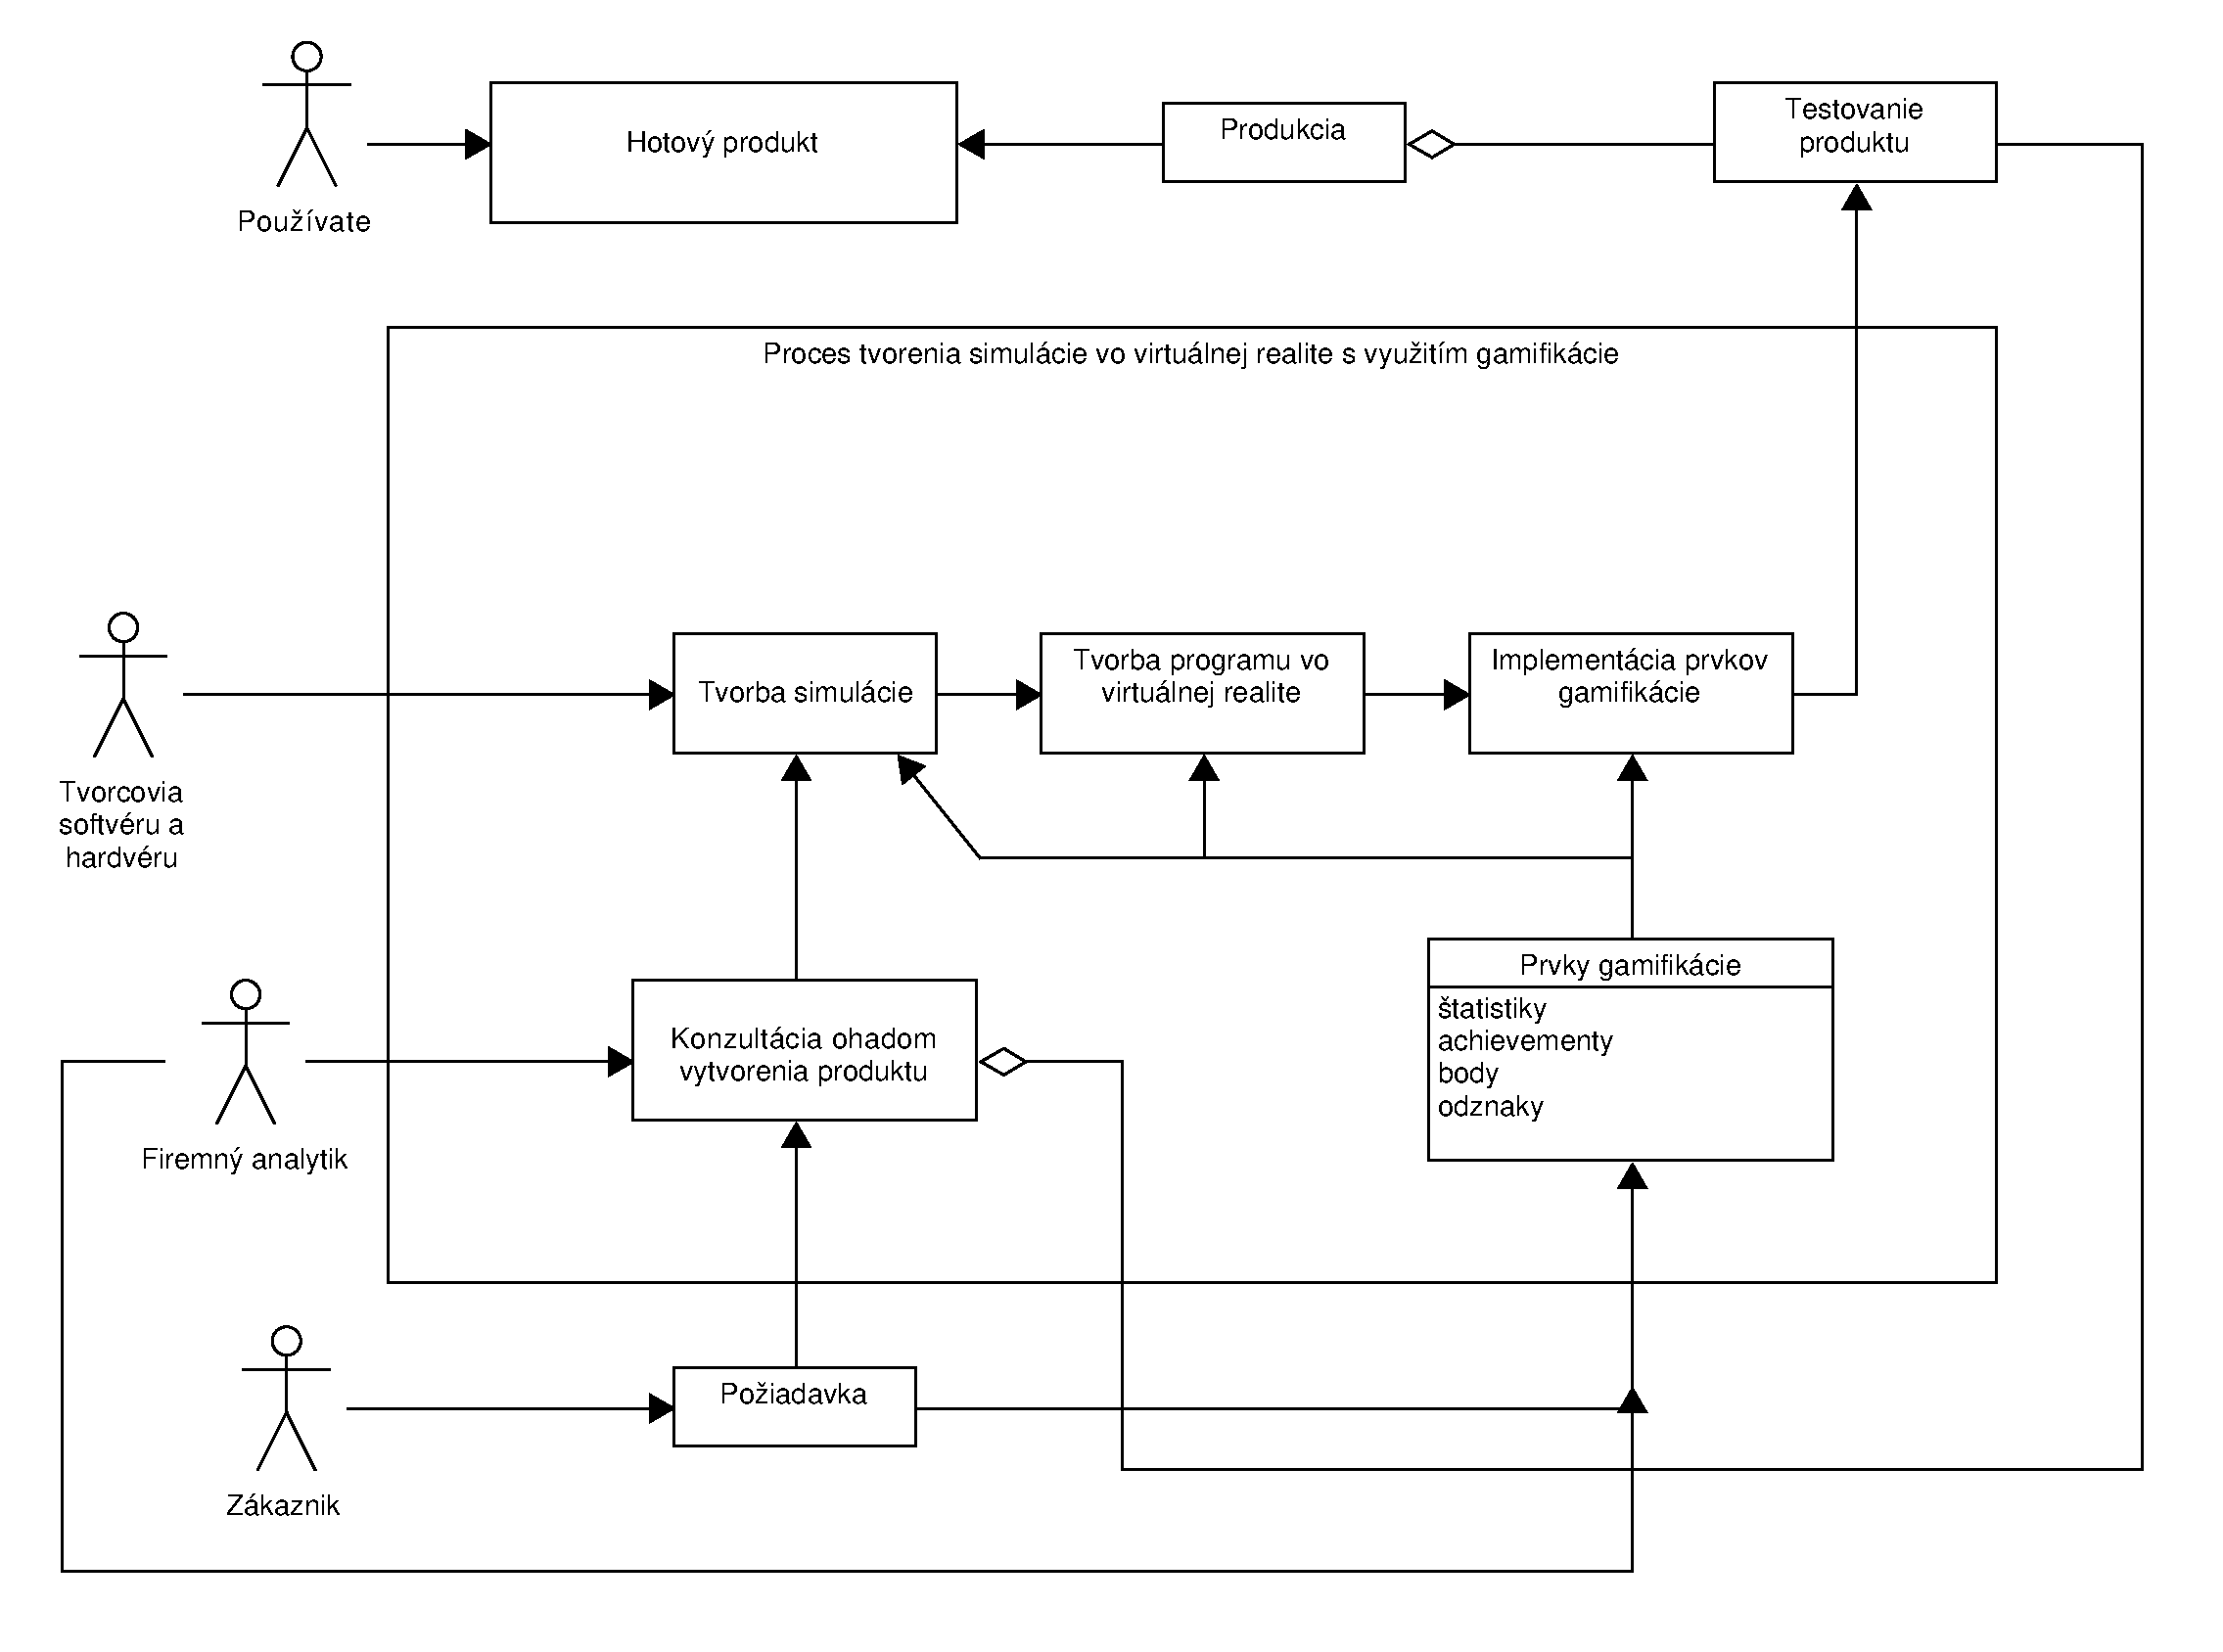
\includegraphics[scale=0.35]{images_article/umlet mip.pdf}
    \caption{Proces tvorenia simulácie vo VR s využitím gamifikácie (P. Sartoris)}
\end{figure}

%obrázok
\begin{figure}[tbhp]
    \centering
   \label{Image1}
    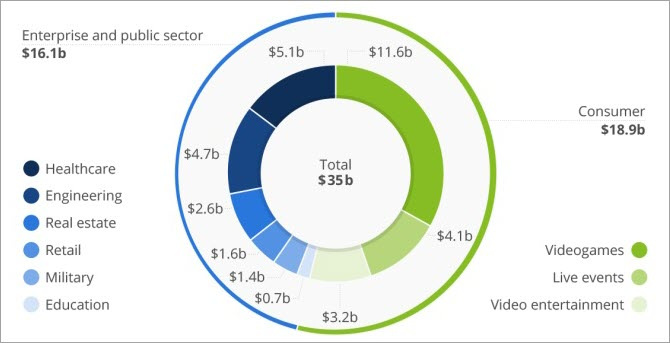
\includegraphics[scale=0.68]{images_article/Potential-of-VR-applications-by-category.jpg}
    \caption{Budúcnosť na trhu virtuálnej reality - potenciál podľa kategórií (zdroj: \url{https://www.softwaretestinghelp.com/future-of-virtual-reality/})}
    \clearpage
\end{figure}

\newpage
%%%%%%%%%%%%%%%%%%%%%%%%%%%%%%%%%%%%%%%%%%%%%%%%%%%%%%%%%%%%%%%%%%%%%%%%%%%%%%%%%%%%
%\clearpage
\bibliography{literature_article}
\bibliographystyle{abbrv}
%%%%%%%%%%%%%%%%%%%%%%%%%%%%%%%%%%%%%%%%%%%%%%%%%%%%%%%%%%%%%%%%%%%%%%%%%%%%%%%%%%%%
\end{document}
%%%%%%%%%%%%%%%%%%%%%%%%%%%%%%%%%%%%%%%%%%%%%%%%%%%%%%%%%%%%%%%%%%%%%%%%%%%%%%%%%%%%
